\documentclass[11pt]{report}
\usepackage[utf8]{inputenc}
\usepackage{amsmath, graphicx, subfiles, float, multirow, listings, subcaption}

\begin{document}

\chapter*{Exercise i}
The equation set to be solved numerically is \begin{equation} \begin{split} \mu \nabla ^2\mathbf{u} &= \nabla p \\ \nabla \cdot \mathbf{u} &= 0 \end{split} \end{equation}

To solve this equation numerically in FEniCS we must first transform it into its variational form. This is achieved by multiplying the equation with a test function, $\mathbf{v}$, and then integrating it over the domain $\Omega$. This gives

\begin{equation}
\begin{split}
\mu \int _\Omega \nabla ^2 \mathbf{u} \cdot \mathbf{v} d\mathbf{x} & = \int _\Omega \nabla p \cdot \mathbf{v} d\mathbf{x} \\
\mu \nabla \mathbf{u}\cdot \mathbf{v} \Big |_{\partial \Omega} - \mu \int _\Omega \nabla \mathbf{u}\cdot \nabla \mathbf{v} d\mathbf{x} &= \int _\Omega \nabla p\cdot \mathbf{v}d\mathbf{x} \\
-\mu \int _\Omega \nabla \mathbf{u}\cdot \nabla \mathbf{v} d\mathbf{x} &= \int _\Omega \nabla p\cdot\mathbf{v}d\mathbf{x}
\end{split}
\end{equation}

I have used the Dirichlet boundary conditions for the test function which leaves us with only two terms, one bilinear and on linear. Usually we would have to use the second equation as well, but for this calculation I have set $\nabla p$ to a constant. Hence I only have one unknown, $\mathbf{u}$, and therefore I only need one equation. To calculate the volume rate I have used the velocity and integrated it over the area of the geometry.\\

For all cases I have used mshr to construct the meshes. The errornorm calculations have been done for first, second and third order polynomials with 4 different mesh sizes. \\

The numerical solution of the velocity fields can be seen in figure 1.

\begin{figure}[htb]
\begin{subfigure}{.3\textwidth}
	\centering
	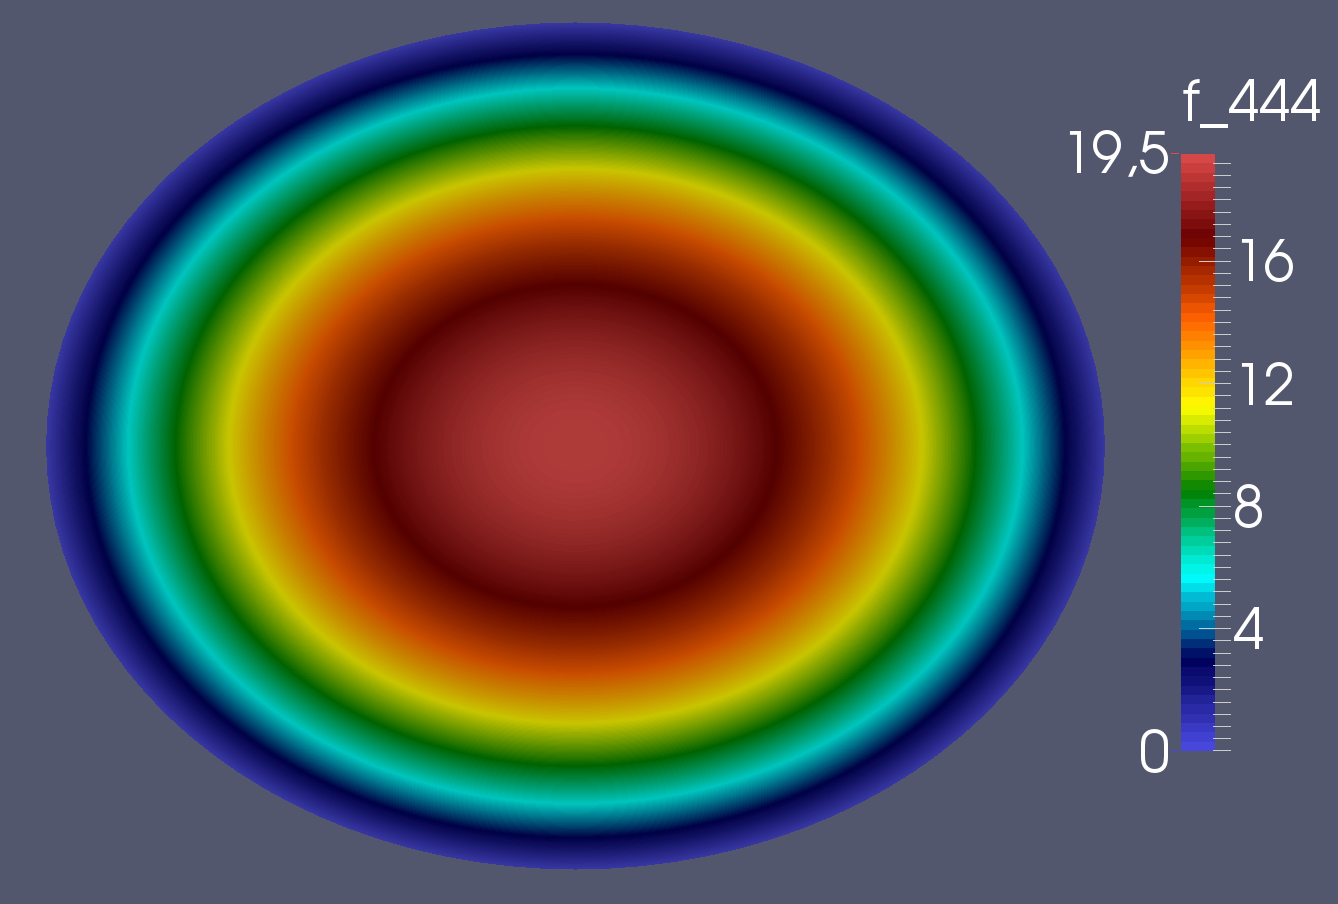
\includegraphics[width=.9\linewidth]{images/ex1_47.png}
\end{subfigure}
\begin{subfigure}{.3\textwidth}
	\centering
	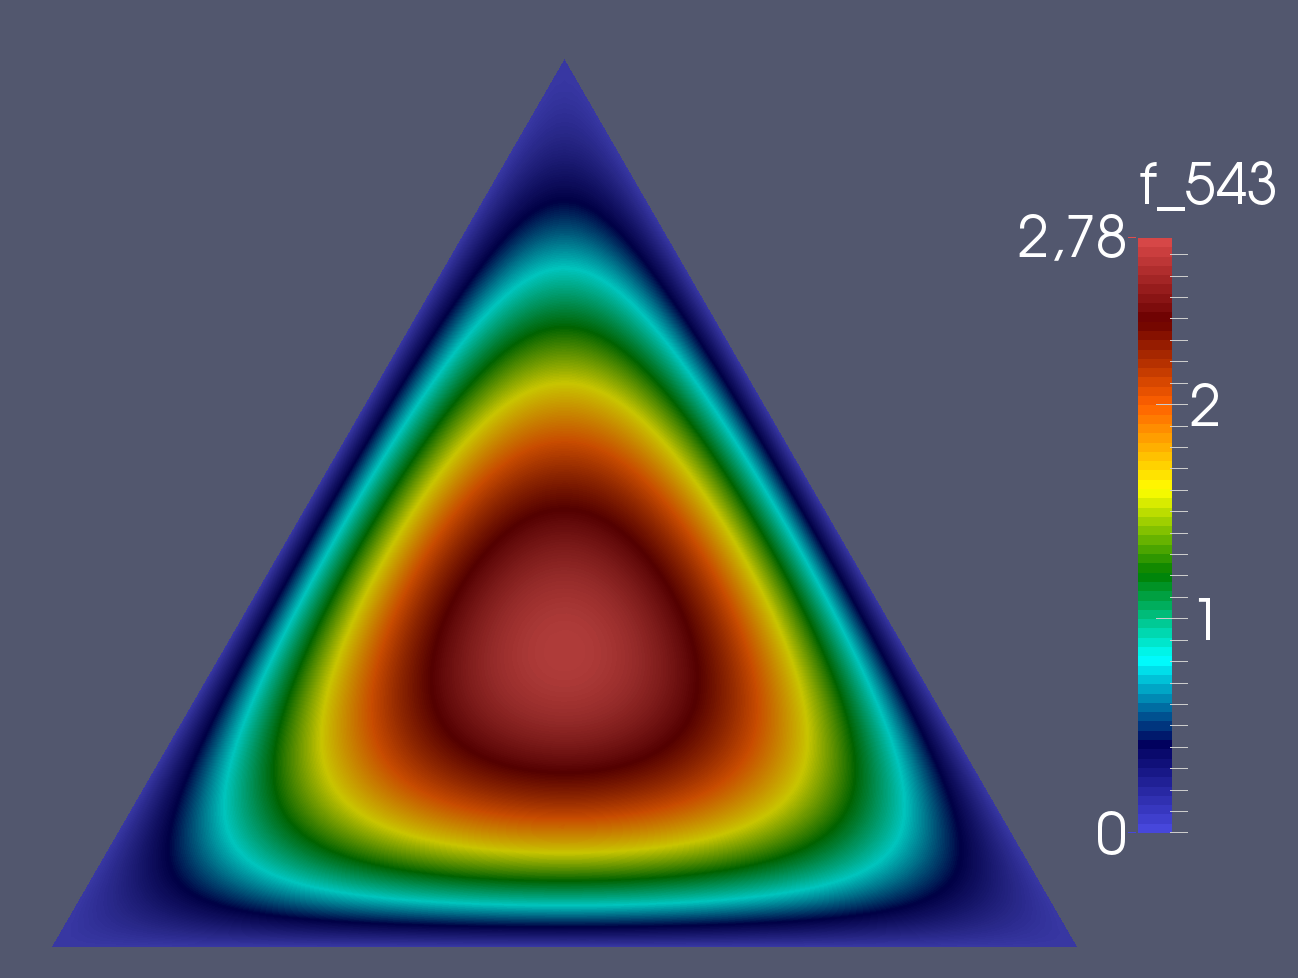
\includegraphics[width=.9\linewidth]{images/ex1_49.png}
\end{subfigure}
\begin{subfigure}{.3\textwidth}
	\centering
	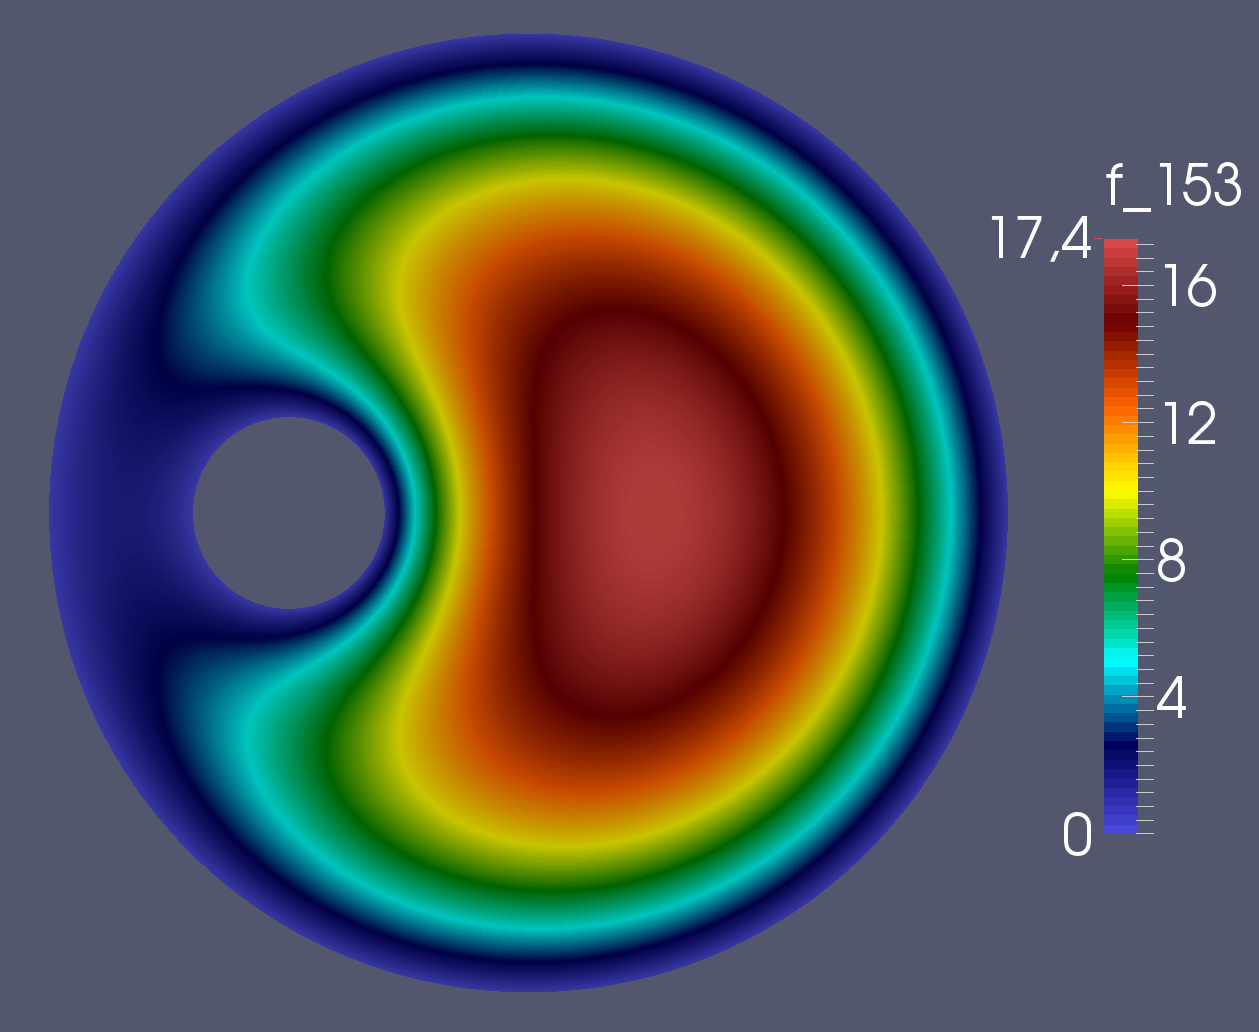
\includegraphics[width=.9\linewidth]{images/ex1_52.png}
\end{subfigure}
\caption{Numerical solution of velocity fields for the different geometries.}
\end{figure}



\section*{Ellipse}

For the ellipse I have set the radius to $(1, 0.8)$.
\begin{figure}[htb]
\begin{center}
\begin{tabular}{|c|c|c|c|}
\hline
Mesh size & P1 Elements & P2 Elements & P3 Elements \\ \hline
0.03847 & 0.19340  & 0.020544 & 0.020475         \\ \hline
0.01923 & 0.042457 & 0.020473 & 0.020473           \\ \hline
0.009618 & 0.015891 & 0.020476 & 0.020485           \\ \hline
0.004809 & 0.018573 & 0.020487 & 0.020493           \\ \hline
\end{tabular}
\end {center}
\caption{Error norm for the velocity field using mesh refining and higher order polynomials.}
\end{figure}

We see that for P1 elements refining the mesh has a positive effect. For the first mesh refinement I get a convergence rate around 2 which is what it should be. For P2 and P3 elements the refining has almost no effect on the solution. This can indicate that the exact solution is of one of these orders. 

\begin{figure}[htb]
\begin{center}
\begin{tabular}{|c|c|c|c|}
\hline
Mesh size & P1 Elements & P2 Elements & P3 Elements \\ \hline
0.03847 & 0.18325  & 0.032692 & 0.032534         \\ \hline
0.01923 & 0.068492 & 0.032535 & 0.032490           \\ \hline
0.009618 & 0.041329 & 0.032490 & 0.032479           \\ \hline
0.004809 & 0.034678 & 0.032479 & 0.032476           \\ \hline
\end{tabular}
\end {center}
\caption{The difference in volume flow rate between the exact solution and the numerical solution.}
\end{figure}


\section*{Triangle}

For the triangle I have set all the sides to length 1.
\begin{figure}[htb]
\begin{center}
\begin{tabular}{|c|c|c|c|}
\hline
Mesh size & P1 Elements & P2 Elements & P3 Elements \\ \hline
0.28867 & 0.19717  & 0.017725 & 1.0408e-07         \\ \hline
0.14433 & 0.053910 & 0.0022174 & 4.6137e-07           \\ \hline
0.072168 & 0.014469 &  0.0002777 & 4.9440e-07           \\ \hline
0.036084 & 0.0035914 & 3.4000e-05 & 4.1326e-07           \\ \hline
\end{tabular}
\end {center}
\caption{Error norm for the velocity field using mesh refining and higher order polynomials.}
\end{figure}

Here we get good results when refining both for P1 and P2 elements. For the P2 elements we get a convergence rate of 2, and for the P2 elements we get a convergence rate of 3. For the P3 elements we get almost no change in results when refining.

\begin{figure}[htb]
\begin{center}
\begin{tabular}{|c|c|c|c|}
\hline
Mesh size & P1 Elements & P2 Elements & P3 Elements \\ \hline
0.28867 & 0.28352  & 0.006098 & 5.9952e-15         \\ \hline
0.14433 & 0.074969 & 0.0003695 & 2.3647e-14           \\ \hline
0.072168 & 0.019166 & 2.2860e-05 & 8.0824e-14           \\ \hline
0.036084 & 0.0046302 & 1.4414e-06 & 3.9390e-13           \\ \hline
\end{tabular}
\end {center}
\caption{The difference in volume flow rate between the exact solution and the numerical solution.}
\end{figure}

\section*{Eccentric annulus}

For this geometry I have set the outer radius to 1, and the radius of the inner circle to 0.2. I have placed it with coordinates $(-0.5, 0)$. For this geometry I get no good convergence rate so I have just collected the absolute value of the error between the numerical flow rate and the exact flow rate. For P1 elements the refining of the mesh reduces the error but for P2 refining of the mesh increases the difference between the numerical and exacct solution. For P3 elements it stays the same. Since I have chosen to have very fine circles, they are defined by many points, the coarsest mesh is already pretty fine. This might be a contributing factor to why the refining have almost no impact.

\begin{figure}[htb]
\begin{center}
\begin{tabular}{|c|c|c|c|}
\hline
Mesh size & P1 Elements & P2 Elements & P3 Elements \\ \hline
0.009417 & 0.222919  & 0.001182 & 0.001812         \\ \hline
0.004708 & 0.053300 & 0.001775 & 0.001821           \\ \hline
0.002354 & 0.011815 & 0.001819 & 0.001823           \\ \hline
0.001177 & 0.0015682 & 0.001823 & 0.001823           \\ \hline
\end{tabular}
\end {center}
\caption{The difference in volume flow rate between the exact solution and the numerical solution.}
\end{figure}

\chapter*{Exercise ii}

The two equations\footnote{eq(148) and eq(150) from lecture notes.} to solve are \begin{equation} F''' + FF'' + 1 - (F')^2 = 0 \end{equation}
\begin{equation} F''' + 2FF'' + 1 - (F')^2 = 0 \end{equation}
with boundary conditions
\begin{equation}\begin{split} F(0) = F'(0) &= 0 \\ F'(\infty) &= 1 \end{split}\end{equation} 

I use the substitution \begin{equation} H = F' \label{eq:sub1} \end{equation}

which leads me to the new equations to solve
\begin{equation} H'' + FH' + 1 - H^2 = 0 \label{ex21}\end{equation}
\begin{equation} H'' + 2FH' + 1 - H^2 = 0 \label{ex22} \end{equation}
with boundary conditions
\begin{equation}\begin{split} F(0) = H(0) &= 0 \\ H(\infty) &= 1 \end{split}\end{equation} 

In this equation set I now have two unknowns so I use equation \ref{eq:sub1} to get two equations. The important thing to remember is that I must use different test functions for the two equations. Equations \ref{ex21} and \ref{eq:sub1} written in its weak form becomes

\begin{equation}
\begin{split}
-\int _\Omega H' Ht'dx + \int _\Omega FH'Htdx + \int _\Omega Htdx - \int _\Omega H^2Htdx &= 0 \\
\int _\Omega HFtdx - \int _\Omega F'Ftdx &= 0
\end{split}
\label{ex2_set1}
\end{equation}

where $Ht$ and $Ft$ are test functions. The second equation set, using equations \ref{ex22} and \ref{eq:sub1}, written on weak form becomes

\begin{equation}
\begin{split}
-\int _\Omega H' Ht'dx + 2\int _\Omega FH'Htdx + \int _\Omega Htdx - \int _\Omega H^2Htdx &= 0 \\
\int _\Omega HFtdx - \int _\Omega F'Ftdx &= 0
\end{split}
\label{ex2_set2}
\end{equation}

\section*{Newton iteration}

When we are using Newton iteration in FEniCS we must remember not to use TrialFunctions. Newton iteration is the default way to solve coupled equations in FEniCS so by just adding the two equations together and splitting them in linear and bilinear terms, I can solve them with the same approach I would use with an uncoupled problem. The error tolerance for the iteration is set to $10^{-10}$ and FEniCS uses 6 iterations to reach this limit for both equation set. The plot of F for equation set \ref{ex2_set1} can be seen in figure \ref{fig:ex2_newton_1}.

\begin{figure}[htb]
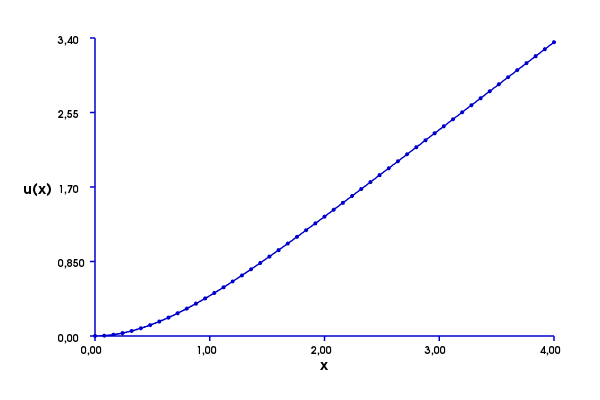
\includegraphics[scale=0.5]{images/ex2_newton_1.png}
\caption{The figure displays the solution of F for equation set \ref{ex2_set1} using Newton iterations.}
\label{fig:ex2_newton_1}
\end{figure}

For equation set \ref{ex2_set2} we can see the plot of F in figure \ref{fig:ex2_newton_2}

\begin{figure}[htb]
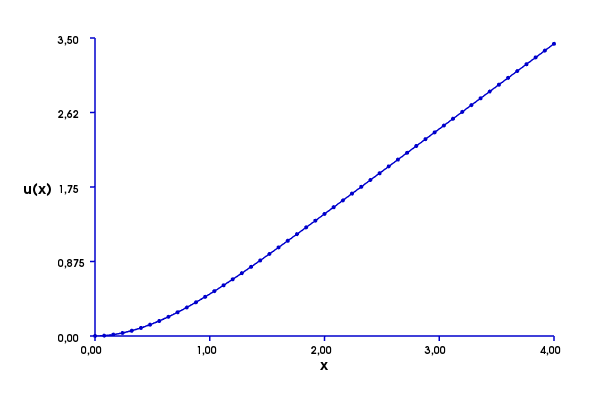
\includegraphics[scale=0.5]{images/ex2_newton_2.png}
\caption{The figure displays the solution of F for equation set \ref{ex2_set2} using Newton iterations.}
\label{fig:ex2_newton_2}
\end{figure}

We see there is a small difference in the maximum value for F. I would assume this comes from the factor 2 that is added to the second term.

\section*{Picard iteration}

When we use Picard iteration we have to do something else with the non linear term. Instead of calculating $H^2$ we make another function $H1$ that we insert as a guess for one of the $H$. We then solve the equation iteratively until $H-H1<\epsilon$ where $\epsilon$ is a small number that is set by the programmer. The maximum size this parameter can have will usually vary from problem to problem but for now I have used $\epsilon = 1e-14$. For equation set \ref{ex2_set1} the solution is the same as for the newton iteration but for equation set \ref{ex2_set2} the solution is not the same at all. I have tried to figure it out, but I have not managed to find out why this happens.

\begin{figure}[htb]
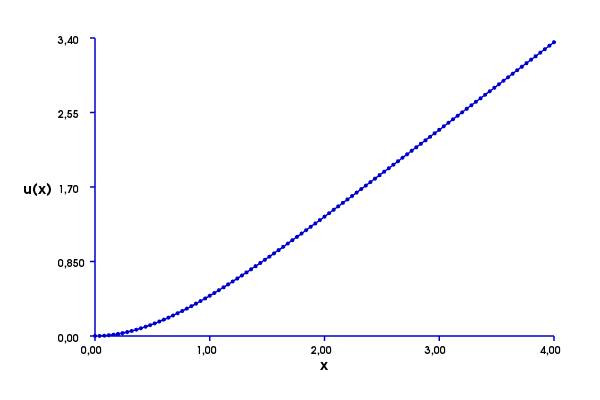
\includegraphics[scale=0.5]{images/ex2_picard_1.png}
\caption{The figure displays the solution of F for equation set \ref{ex2_set1} using Picard iterations.}
\label{fig:ex2_newton_2}
\end{figure}

\begin{figure}[htb]
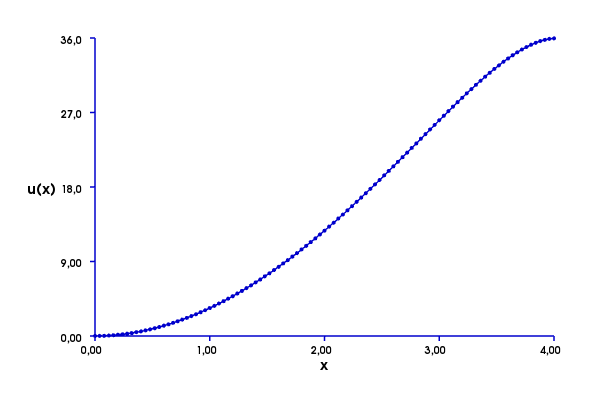
\includegraphics[scale=0.5]{images/ex2_picard_2.png}
\caption{The figure displays the solution of F for equation set \ref{ex2_set2} using Picard iterations. Solution is very different from the others.}
\label{fig:ex2_newton_2}
\end{figure}

\chapter*{Exercise iii}

Viscous flows where the Reynolds number is very low, so called laminar flow, is often referred to as Stokes flow. When the Reynolds number is much less than 1 we can assume that the acceleration terms in the Navier-Stokes equation can be neglected. The Navier-Stokes equation then simplifies to

\begin{equation}
\begin{split}
\mu \nabla ^2 \mathbf{u} &= \nabla p \\
\nabla \cdot \mathbf{u} &= 0
\end{split}
\end{equation}

The method used for solving these equations are a coupled system where both $\mathbf{u}$ and $p$ are solved as trialfunctions simultaneously using MixedFunctionSpace in FEniCS. First, we obtain the weak formulation of the equations. To do this, I multiply with a test function $\mathbf{v}$ and integrate over the domain $\Omega$.

\begin{equation}
\begin{split}
\mu \int _\Omega \nabla ^2 \mathbf{u} \cdot \mathbf{v} d\mathbf{x} & = \int _\Omega \nabla p \cdot \mathbf{v} d\mathbf{x} \\
\mu \nabla \mathbf{u}\cdot \mathbf{v} \Big |_{\partial \Omega} - \mu \int _\Omega \nabla \mathbf{u}\cdot \nabla \mathbf{v} d\mathbf{x} &= p\mathbf{v} \Big |_{\partial \Omega} - \int _\Omega p\nabla \mathbf{v}d\mathbf{x} \\
\mu \int _\Omega \nabla \mathbf{u}\cdot \nabla \mathbf{v} d\mathbf{x} &= \int _\Omega p\nabla \mathbf{v}d\mathbf{x}
\end{split}
\end{equation}
The second equation is multiplied with a test function $q$
\begin{equation}
\int _\Omega q\nabla \cdot \mathbf{u} d\mathbf{x} = 0
\end{equation}

I calculate the velocity- and pressure field with a standard FEniCS solver and then use the Cauchy-Riemann equations to obtain the stream functions, which can be seen in figure \ref{fig:ex3}.

\begin{figure}[htb]
\center
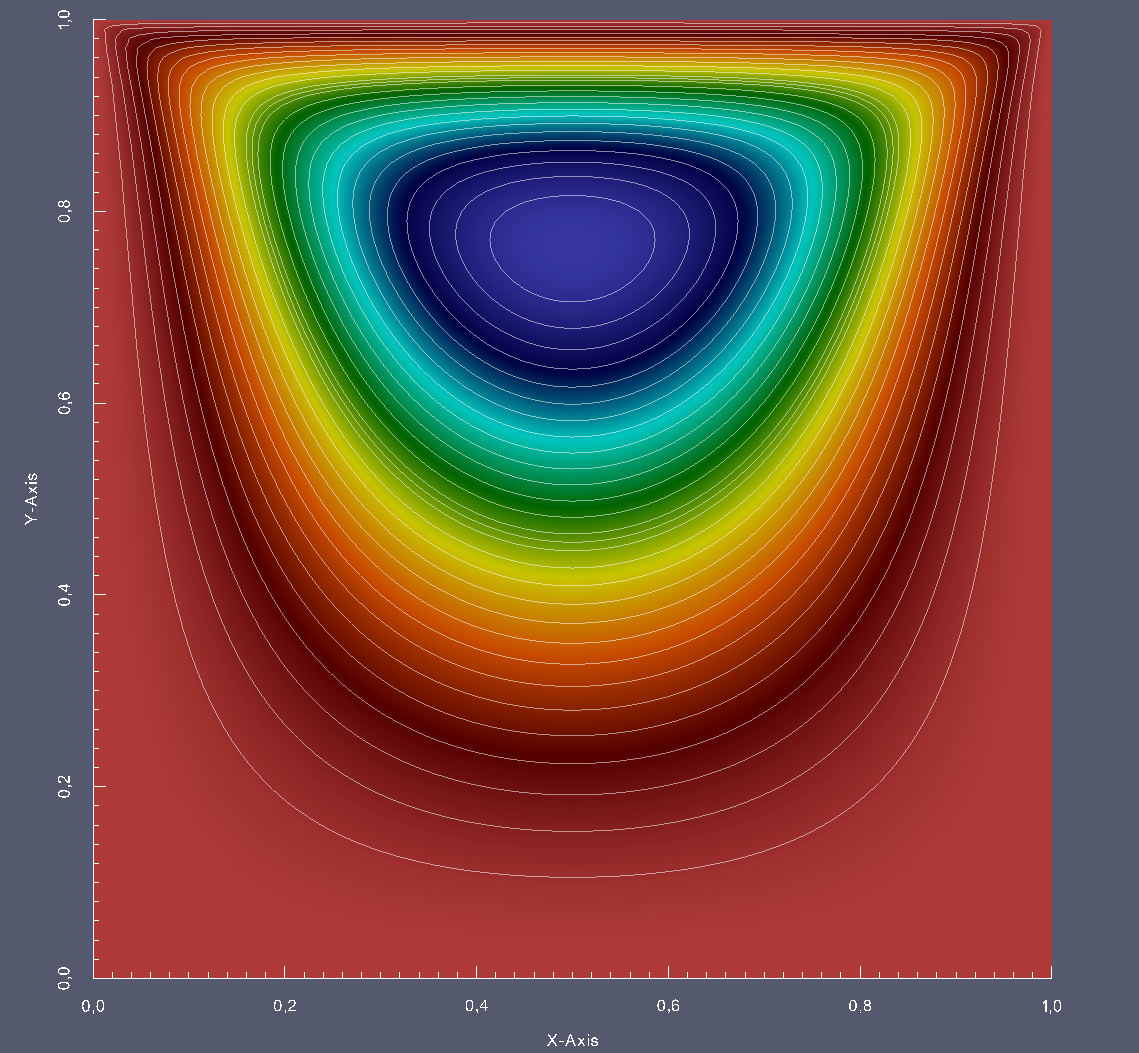
\includegraphics[scale=0.2]{images/ex3_streamfunction.png}
\caption{Plot of the stream function. The blue area depicts the center of the vortex.}
\label{fig:ex3}
\end{figure}

Reading from the axis gives us an idea about the coordinates for the center of the vortex. Using python to calculate it returns
\begin{verbatim}
Coordinates for center of vortex: 
x = 0.5, y = 0.765

\end{verbatim}


\chapter*{Exercise iv}

\section*{Task a}

\begin{figure}[htb]
\begin{center}
\begin{tabular}{|c|c|c|}
\hline
Mesh size & x coordinates & y coordinates \\ \hline
0.111038 & 0.0  & 0.1           \\ \hline
0.084445 & 0.4  & 0.1            \\ \hline
0.051954 & 0.521767 & 0.0466142            \\ \hline
0.009721 & 0.534367 & 0.0380688           \\ \hline
0.004086 & 0.534517 & 0.0378999           \\ \hline
0.000816 & 0.535267 & 0.0392285           \\ \hline
\end{tabular}
\end {center}
\caption{Coordinates for center of vortex depending on mesh size.}
\end{figure}


\section*{Task b}

The contour plot can be seen in figure \ref{fig:ex4b}

\begin{figure}[htb]
\center
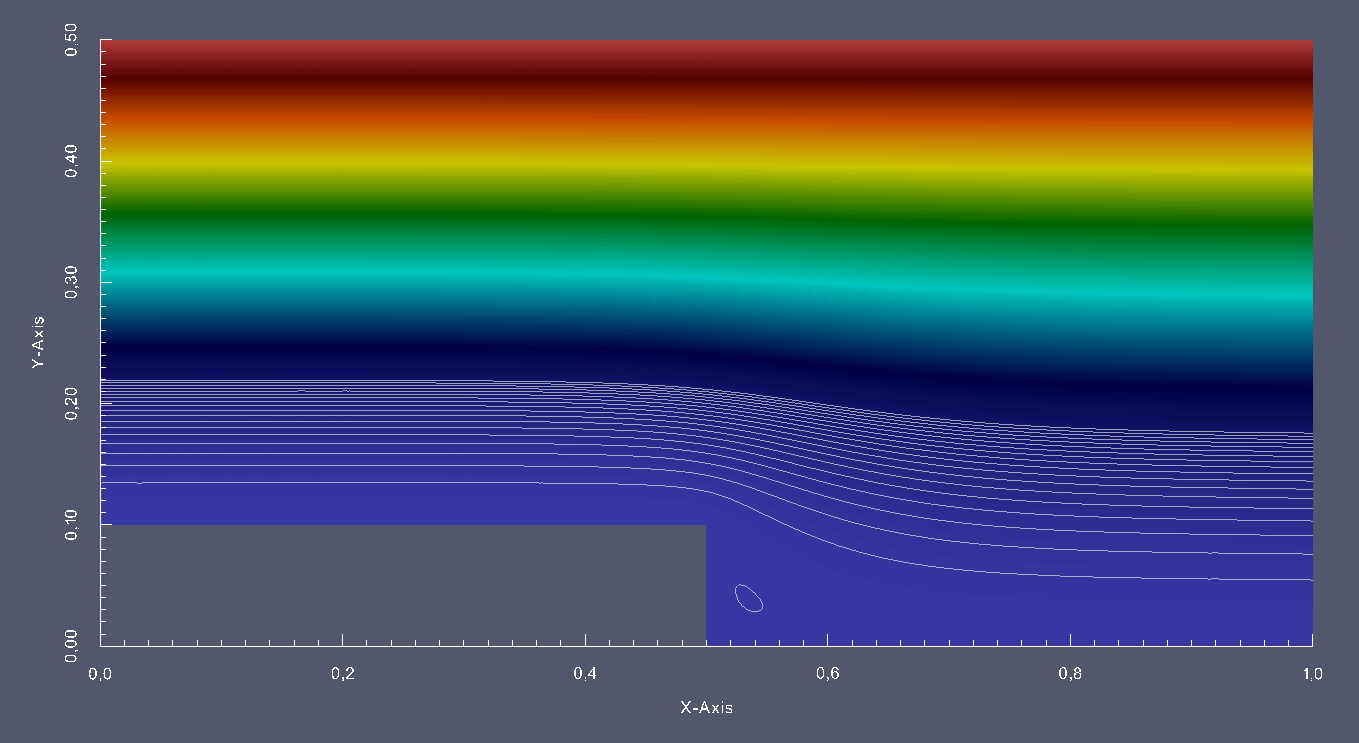
\includegraphics[scale=0.2]{images/ex4a_psi.png}
\caption{Contour plot of stream function. The vortex can be seen next to the step.}
\label{fig:ex4b}
\end{figure}






\section*{Task c}

Calculating the velocity flux in python I get
\begin{verbatim}
Velocity flux inn: 0.212596220711
Velocity flux out: 0.212596220711
Flux error: -8.04911692853e-16

\end{verbatim}

This indicates that mass is conserved.

\section*{Task d}

Calculating with python returns
\begin{verbatim}
Coordinates for center of vortex: 
x = 0.535267, y = 0.0392285

\end{verbatim}

which is exactly the same I got for the plate moving in the positive x-direction. For a creeping flow, the direction of the flow is not the main factor for where the vortex is located. It is the geometry that decides where the vortex should be.

\section*{Task e}

The stress tensor includes a term for the shear stress. To compute the normal stress I can skip calculating this. Calculating with python I get
\begin{verbatim}
Normal stress: 121.373999197
\end{verbatim}

If I turn the direction of the flow I get the same normal stress but with a different sign.

\end{document}
